\documentclass{beamer}

\usetheme{Hannover}
\setbeamertemplate{footline}[frame number]

\setbeamertemplate{blocks}[rounded]%
[shadow=false]

\setbeamercolor{block title}{fg=black,bg=blue!20}    
\setbeamercolor{block body}{fg=black,bg=blue!10}      
\setbeamercolor{block body alerted}{fg=white,bg=red}

\definecolor{myblue}{RGB}{1,15,150}

% % definition by cases in equations
% %% The environment cases* handles the second column as text
\usepackage{mathtools}
% Options for hyperref
\hypersetup{
  colorlinks = true,
  linkcolor = myblue,
  urlcolor = magenta
}

\title{The STOC free model}
\subtitle{Objectives, hypotheses and model overview}
\author[Madouasse \textit{et al.}]{Aurélien Madouasse \texorpdfstring{\\}{}\& \texorpdfstring{\\}{}the STOC free consortium}
\institute{\url{https://www.stocfree.eu/}}

%\titlegraphic{
\includegraphics[width=\textwidth]{imgs/title_page_bg.png}}


\begin{document}
{
%  \usebackgroundtemplate{
\includegraphics[width=\paperwidth]{imgs/title_page_bg1.png}}%
  \usebackgroundtemplate{
\includegraphics[width=1.1\paperwidth]{imgs/title_page_bg1.png}}%
  \maketitle
}

\begin{frame}
\frametitle{Table of Contents}
  \tableofcontents
\end{frame}  

\section{Context and objectives}

\begin{frame}
\frametitle{Table of Contents}
  \tableofcontents[currentsection]
\end{frame}  


\begin{frame}
\frametitle{Infectious diseases of cattle}
\framesubtitle{Regulated diseases}
\begin{itemize}
  \item{Public health threats}
  \item[]{\scriptsize e.g. Tuberculosis}
  \item{Economic impact}
  \item[]{\scriptsize e.g. Foot and mouth disease}
  \item{Legislation on how to perform surveillance in order to substantiate freedom from disease}
  \item{Every country performs surveillance in the same way $\rightarrow$ comparable output}
  \item[$\Rightarrow$]{\textcolor{red}{\textbf{Input-based surveillance}}}
 \end{itemize}
\end{frame}

\begin{frame}
\frametitle{Infectious diseases of cattle}
\framesubtitle{Non-regulated diseases}
 \begin{itemize}
  \item{A lot of important infectious diseases are not regulated but have regional / national control programmes in place}
  \item[]{\scriptsize e.g. BVD, paratuberculosis $\ldots$}
  \begin{itemize}
   \item{No \emph{legal} prescription on the way to perform surveillance}
   \item{Important diversity in the design of surveillance programmes}
   \item{The \emph{free status} in one programme can have a different meaning than the \emph{free status} in another programme}
  \end{itemize}
  \item[$\Rightarrow$]{Creates difficulties when trading animals between herds enrolled in different programmes}
  \item[$\Rightarrow$]{\textcolor{red}{\textbf{Output-based surveillance}}: production of an output that is comparable regardless of the input surveillance data}
    \end{itemize}
\end{frame}

\begin{frame}
\frametitle{A method for output-based surveillance}
\begin{itemize}
\item{Need for a method taking inputs from diverse surveillance programmes able to produce an output that is comparable}
  \begin{itemize}
   \item{Structure of the method/model determined by what is common across surveillance programmes}
   \item{Probability of freedom from infection estimated in a given programme from:}
   \begin{itemize}
    \item{surveillance data available in the programme}
    \item{relevant knowledge (e.g. test characteristics)}
   \end{itemize}
  \end{itemize}
\end{itemize}
\end{frame}

\begin{frame}
\frametitle{Control programmes}
\framesubtitle{Common features}
\begin{itemize}
 \item{\emph{Control} programmes against cattle non-regulated diseases: prevalence $>0$}
 \item{Objective: disease control or eradication}
 \item{Organised at regional or country level}
 \item{Rely on a surveillance component for the identification of infected herds or animals}
 \item{Detection of infection followed by control phase}
 \item{Surveillance performed in all participating herds}
 \item{Herd tested repeatedly over time}
  \begin{itemize}
   \item[$\Rightarrow$]{Longitudinal data}
  \end{itemize}
\end{itemize}
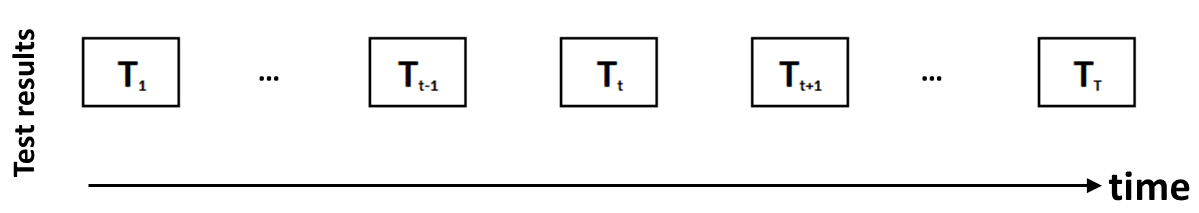
\includegraphics[width=\textwidth]{imgs/longitudinal_data.png}
\end{frame}

\begin{frame}
\frametitle{Control programmes}
\framesubtitle{Common features}
\begin{itemize}
 \item{Tests are imperfect}
 \begin{itemize}
  \item{Sensitivity: $Se = p(T^+|D^+) < 1$}
  \item{Specificity: $Sp = p(T^-|D^-) < 1$}
 \end{itemize}
 \item[$\Rightarrow$]{Uncertainty in the true status of tested animals / herds}
\end{itemize}
\center
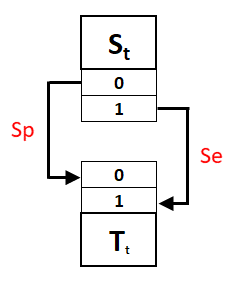
\includegraphics[width=.3\textwidth]{imgs/SeSp.png}
\end{frame}


\section{Modelling framework}
\begin{frame}
\frametitle{Table of Contents}
  \tableofcontents[currentsection]
\end{frame} 

\begin{frame}
\frametitle{Modelling objectives}
\begin{itemize}
 \item{Objective: Predict herd level probabilities of \emph{(freedom from)} infection from longitudinal test data collected as part of surveillance programmes against endemic infectious diseases of cattle}
 \item{The modelling framework should:}
 \begin{itemize}
  \item{Allow the use of longitudinal data i.e. account for the fact that sequences of test results are not random}
  \item{Account for imperfect test information}
 \end{itemize}
\end{itemize}
\end{frame}

\begin{frame}
\frametitle{Hidden Markov models}
\begin{itemize}
 \item{Hidden Markov Models (\textbf{HMM}s) model a latent discrete variable with a Markovian dynamics, whose state at a given time determines the distribution of an observed variable}
  \begin{itemize}
   \item{\textbf{discrete variable}: the variable of interest can be in 1 of $k$ states. In the STOC free model, $k=2$ (positive or negative status)}
   \item{\textbf{latent variable}: this discrete variable is not directly observed. In the STOC free model, the \textbf{latent status} determines the probability of a negative or positive test result through test sensitivity and specificity}
   \item{\textbf{Markovian dynamics}: the latent status is modelled in discrete time steps. The latent status at time $t$ only depends on the status at time $t-1$. The probabilities of transition between the $k$ states between 2 time points are described by a $k$ x $k$ transition matrix.}
  \end{itemize}
\end{itemize}
\end{frame}

\begin{frame}
\frametitle{Representation of surveillance programmes as HMMs}
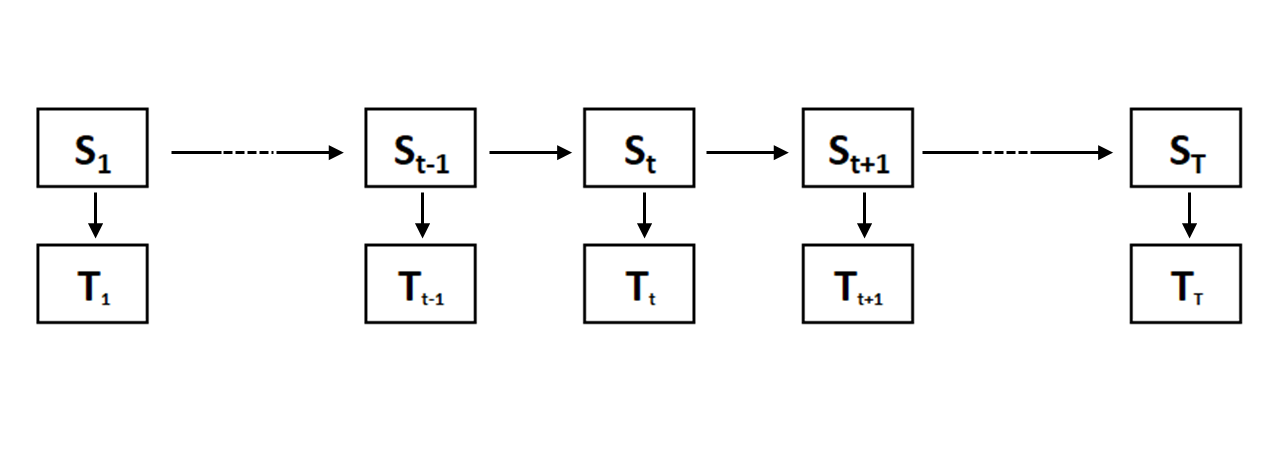
\includegraphics[width = \textwidth]{imgs/surveillance_programmes_HMMs.png}
\begin{itemize}
 \item{$S_t$: latent status of interest at time $t$ , from $t=1$ to $t=T$}
 \item{$T_t$: test result at time $t$}
\end{itemize}
\end{frame}

\begin{frame}
\frametitle{Representation of surveillance programmes as HMMs}
\framesubtitle{Status dynamics}
\begin{columns}
\begin{column}{0.6\textwidth}
\begin{itemize}
  \item{Time steps of equal duration}
  \begin{itemize}
   \item[]{\scriptsize(Discrete-time model)}
  \end{itemize}
  \item{Herd status at time $t$ depends on herd status at time $t_1$}
  \begin{itemize}
   \item[]{\scriptsize(Markovian property)}
  \end{itemize}
\end{itemize}
\vspace{.5cm}
$$S_t \sim Bernoulli(\pi_t)$$
$$\pi_t = \begin{cases*} \tau_1 &if $S_{t-1}=0$ \\
                        \tau_2 &if $S_{t-1}=1$ \end{cases*}$$
\end{column}
\begin{column}{0.4\textwidth}
\vspace{2cm}
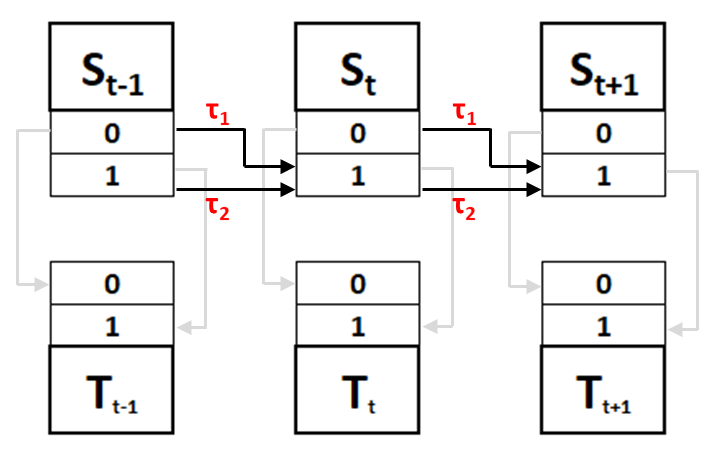
\includegraphics[width = 1.1\textwidth]{imgs/dynamics.png}
\end{column}
\end{columns}
\end{frame}

\begin{frame}
\frametitle{Representation of surveillance programmes as HMMs}
\framesubtitle{Status dynamics}
\begin{columns}
\begin{column}{0.6\textwidth}
\begin{itemize}
  \item{Herd level probability of new infection ($\tau_{1t}$) modelled as a function of one or several risk factors ($X_t$) using logistic regression}
\end{itemize}
\vspace{.5cm}
$$ln(\frac{\tau_{1t}}{1 - \tau_{1t}}) = X_{t} \theta$$
\end{column}
\begin{column}{0.4\textwidth}
\vspace{2cm}
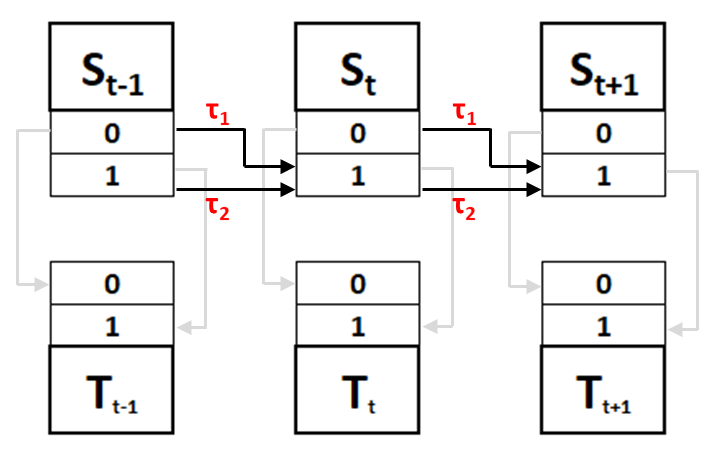
\includegraphics[width = 1.1\textwidth]{imgs/dynamics.png}
\end{column}
\end{columns}
\end{frame}

\begin{frame}
\frametitle{Representation of surveillance programmes as HMMs}
\framesubtitle{Status dynamics}
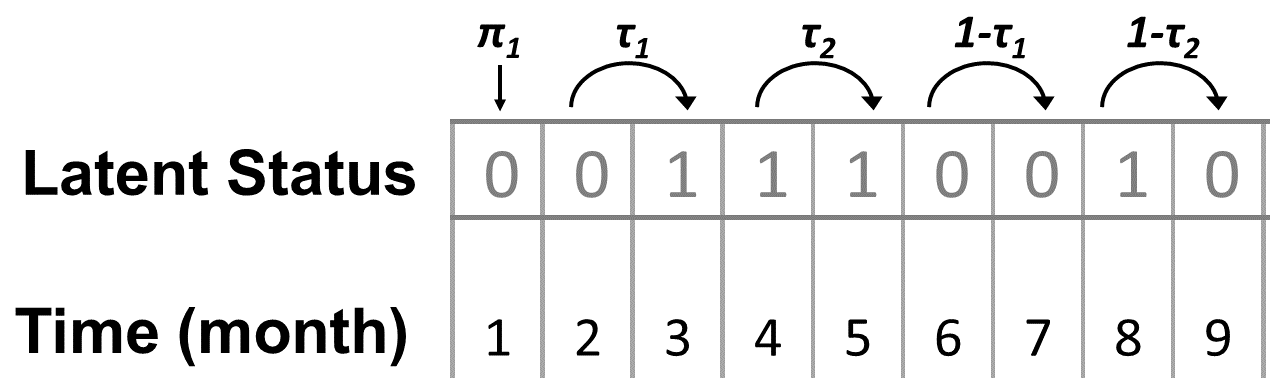
\includegraphics[width = \textwidth]{imgs/infection_dynamics.png}
\end{frame}

\begin{frame}
\frametitle{Representation of surveillance programmes as HMMs}
\framesubtitle{Test results}
\begin{columns}
\begin{column}{0.85\textwidth}
\begin{itemize}
  \item{Herd status at time t is either negative (0) OR positive (1)}
\vspace{2cm}
  \item{Test result at time t is either negative (0) OR positive (1)}
\end{itemize}
\end{column}
\begin{column}{0.15\textwidth}
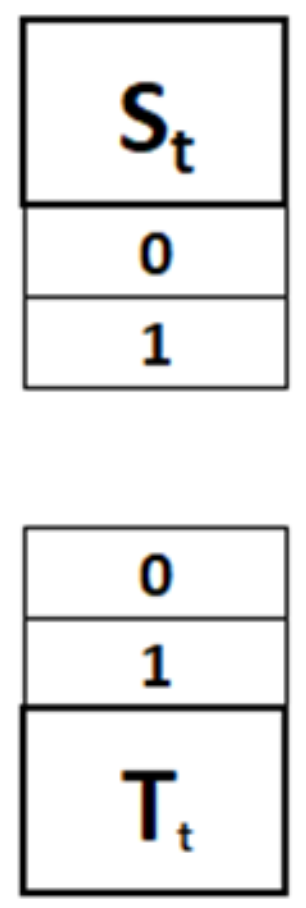
\includegraphics[width = 1\textwidth]{imgs/status_test.png}
\end{column}
\end{columns}
\end{frame}

\begin{frame}
\frametitle{Representation of surveillance programmes as HMMs}
\framesubtitle{Test results}
\begin{columns}
\begin{column}{0.6\textwidth}
\begin{itemize}
  \item{Test results at the herd level}
  \item{Test results depend on the latent status through sensitivity and specificity}
\end{itemize}
\vspace{.5cm}
$$p(T_t = 1) = \begin{cases*} 1 - Sp &if $S_{t}=0$ \\
                              Se &if $S_{t}=1$ \end{cases*}$$
\end{column}
\begin{column}{0.4\textwidth}
\vspace{2cm}
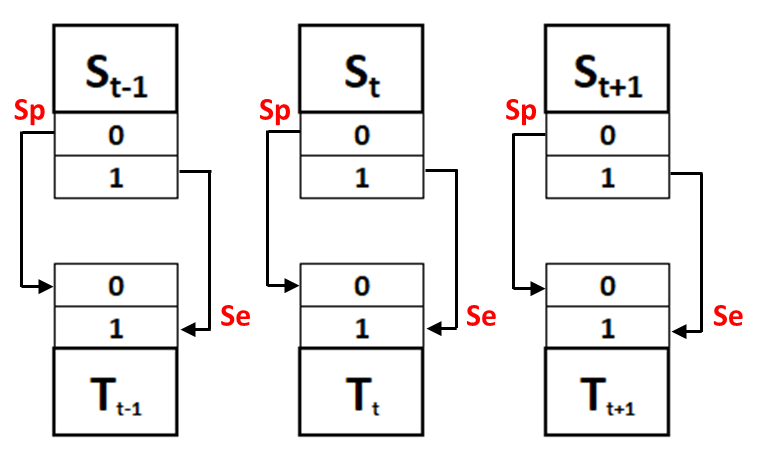
\includegraphics[width = 1.1\textwidth]{imgs/status_test1.png}
\end{column}
\end{columns}
\end{frame}

\begin{frame}
\frametitle{Representation of surveillance programmes as HMMs}
\framesubtitle{Test results}
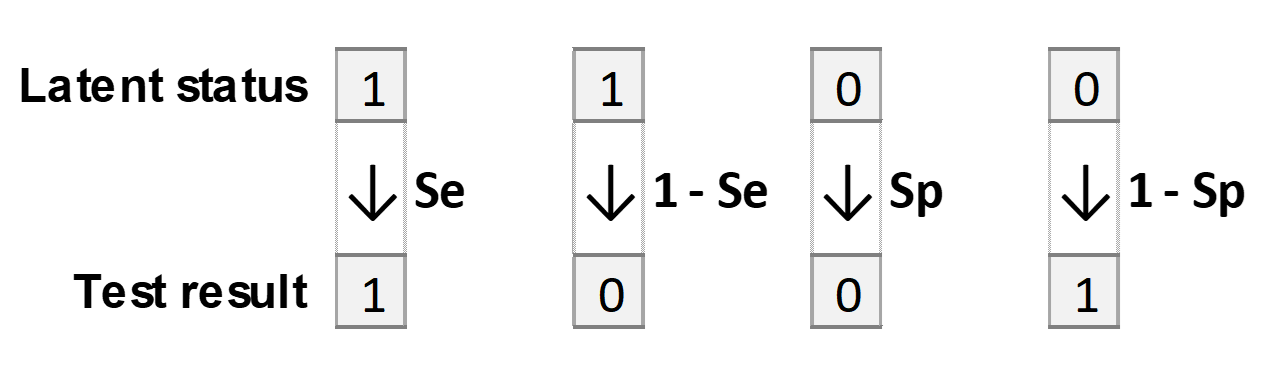
\includegraphics[width = \textwidth]{imgs/test_imperfection.png}
\end{frame}

\begin{frame}
\frametitle{Predictions}

\begin{itemize}
 \item{The model predicts a herd level probability of being status positive at time $T$}
 \item{All the data available up to $T$ are used for paremeter estimation}
\end{itemize}
\vspace{.5cm}
\center
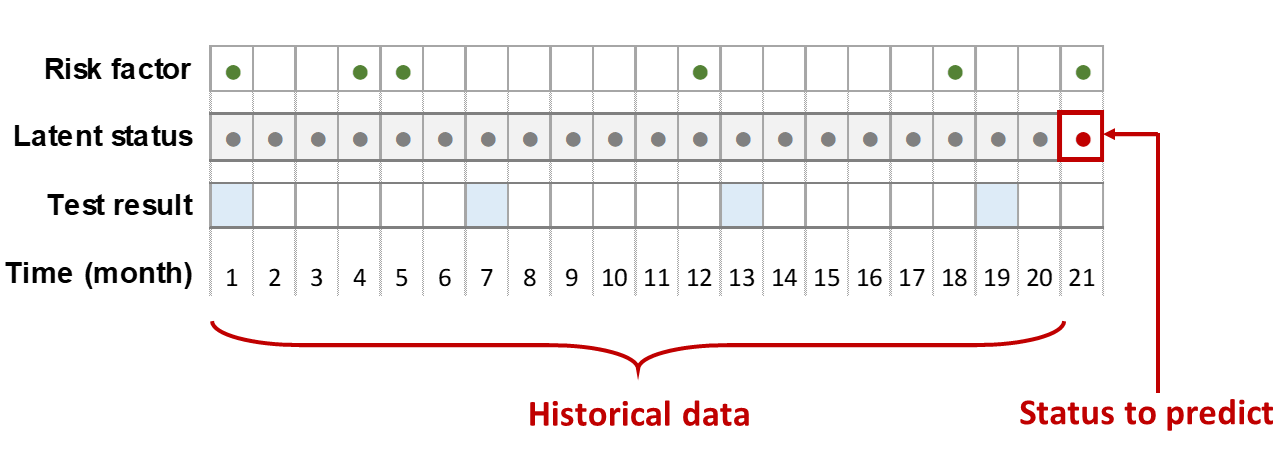
\includegraphics[width = \textwidth]{imgs/modelling_framework.png}
\end{frame}

\begin{frame}
\frametitle{Summary of the different model parameters}
\begin{itemize}
 \item{$\pi_1$: probability of being status positive on the first test month}
 \item{$\tau_1$: probability of becmoing status positive between 2 months}
 \item{$\theta_1, \theta_2 \ldots$: coefficients of the logistic regression for the probability of becoming status positive}
 \item{$\tau_2$: probability of remaining status positive between 2 months}
 \item{$Se$: herd-level test sensitivity}
 \item{$Sp$: herd-level test specificity}
\end{itemize}
\end{frame}

\begin{frame}
\frametitle{The complete model - no risk factor}
$$S_1 \sim Bernoulli(\pi_1)$$
$$S_t \sim Bernoulli(\pi_t) \hspace{.25cm} \forall t > 1$$
$$\pi_t = \begin{cases*} \tau_1 &if $S_{t-1}=0$ \\
                        \tau_2 &if $S_{t-1}=1$ \end{cases*}$$
$$T_t \sim Bernoulli(p(T_t))$$
$$p(T_t) = \begin{cases*} 1 - Sp &if $S_t = 0$ \\
                         Se &if $S_t = 1$ \end{cases*}$$
\end{frame}

\begin{frame}
\frametitle{The complete model - with risk factors}

$$S_1 \sim Bernoulli(\pi_1)$$
$$S_t \sim Bernoulli(\pi_t) \hspace{.25cm} \forall t > 1$$
$$\pi_t = \begin{cases*} \tau_{1t} &if $S_{t-1}=0$ \\ 
                        \tau_2 &if $S_{t-1}=1$ \end{cases*}$$
$$ln(\frac{\tau_{1t}}{1- \tau_{1t}}) = X_{ht} \theta$$                   
$$T_t \sim Bernoulli(p(T_t))$$
$$p(T_t) = \begin{cases*} 1 - Sp &if $S_t = 0$ \\
                         Se &if $S_t = 1$ \end{cases*}$$
\end{frame}


\section[Estimation \& prediction]{Parameter estimation and status prediction}
\begin{frame}
\frametitle{Table of Contents}
  \tableofcontents[currentsection]
\end{frame} 


\begin{frame}
\frametitle{Data, hypotheses and parameters}
\begin{itemize}
 \item{Data: test results, risk factors}
 \item{What we need to know: probability of infection on the current month}
 \item{What we know (more or less): test characteristics, characteristics of infection dynamics $\ldots$}
 \item{The modelling framework needs to be able to predict herd level probabilities of infection from test results and knowledge about test characteristics}
 \item{Chosen approach: Bayesian inference}
\end{itemize}
\end{frame}

\begin{frame}
\frametitle{Bayes’ theorem}
\begin{itemize}
 \item{What is a conditional probability?}
 \begin{itemize}
  \item{Probability of an event given that another event has already happened}
 \end{itemize}
  \medskip
  \item[]{\textbf{Sensitivity} = probability of a positive test result ($T^+$) given that ($|$) an individual is diseased ($D^+$)}
$$Se = p(T^+|D^+)$$
  \item[]{\textbf{Positive predictive value} = probability that an individual is diseased given a positive test result}
  $$PPV = p(D^+|T^+)$$
\end{itemize}
\end{frame}

\begin{frame}
\frametitle{Bayes’ theorem}
\begin{itemize}
 \item{What is Bayes’ theorem?}
 \begin{itemize}
  \item{A simple formula that relates $p(B|A)$ to $p(A|B)$}
 \end{itemize}
\end{itemize}
\vspace{1.5cm}
\huge
$$p(B|A)=\frac{p(A|B)p(B)}{p(A)}$$
\end{frame}

\begin{frame}
\frametitle{Bayes’ theorem}
\begin{itemize}
 \item{Bayes’ theorem applied to determining the probability of disease given a positive test result}
 \begin{itemize}
  \item{Usually we know test sensitivity, and we would like to know the probability that disease is present given test result}
 \end{itemize}
\end{itemize}
\vspace{1cm}
\begin{large}
$$p(D^+|T^+)=\frac{p(T^+|D+)p(D^+)}{p(T^+)}$$
\end{large}
\begin{itemize}
 \item[-]{$p(D^+|T^+)$: Positive predictive value}
 \item[-]{$p(T^+|D+)$: Test sensitivity}
 \item[-]{$p(D^+)$: Disease prevalence}
 \item[-]{$p(T^+)$: Probability of a positive test}
\end{itemize}
\end{frame}

\begin{frame}
\frametitle{Bayes’ theorem}
\begin{itemize}
 \item{Bayes’ theorem applied to determining the probability of disease given a positive test result}
\end{itemize}
\vspace{.5cm}
$$p(D^+|T^+)=\frac{p(T^+|D+)p(D^+)}{p(T^+)}$$
\pause
\vspace{.5cm}
$$p(D^+|T^+)=\frac{p(T^+|D+)p(D^+)}{p(T^+|D+)p(D^+)+p(T^+|D^-)p(D^-)}$$
\pause
\vspace{.5cm}
$$p(D^+|T^+)=\frac{Se \pi}{Se \pi + (1-Sp)(1-\pi)}$$
\end{frame}


\begin{frame}
\frametitle{Bayes’ theorem}
\framesubtitle{Bayes’ theorem applied to statistical inference}
 \begin{itemize}
  \item{We have some data ($y$) and a model, we would like to know what is the probability of the model parameter ($\theta$) values given these data}
 \end{itemize}
\begin{large}
$$p(\theta|y)=\frac{p(y|\theta)p(\theta)}{p(y)}$$
\end{large}
\begin{itemize}
 \item[$p(\theta|y)$]{Probability of parameters given data $\rightarrow$ \textbf{Posterior distribution}}
 \item[$p(y|\theta)$]{Probability of data given parameters $\rightarrow$ \textbf{Likelihood function}}
 \item[$p(\theta)$]{Parameter prior distributions$\rightarrow$ \textbf{priors}}
 \item[$p(y)$]{\textbf{Normalising constant}}
 \end{itemize}
\end{frame}

\begin{frame}
\frametitle{Bayes’ theorem}
\framesubtitle{Bayes’ theorem applied to statistical inference}
 \begin{itemize}
  \item{Bayesian inference is a way to estimate model parameters incorporating:}
 \begin{itemize}
  \item{data}
  \item{prior knowledge/hypotheses about the model parameters}
 \end{itemize}
\end{itemize}
\end{frame}

\begin{frame}
\frametitle{Bayes’ theorem}
\framesubtitle{Bayes’ theorem applied to statistical inference}
\begin{itemize}
 \item{The normalising constant $p(y)$:}
 \begin{itemize}
  \item{is an integral that cannot be readily computed, except in simple cases}
  \item{makes the area under the posterior density curve sum to 1}
  \item{is a constant}
 \end{itemize}
\end{itemize}
\vspace{.5cm}
\Large
$$p(y)=\int p(y|\theta)p(\theta)d\theta$$
\end{frame}

\begin{frame}
\frametitle{Bayes’ theorem}
\framesubtitle{Bayes’ theorem applied to statistical inference}
\begin{itemize}
 \item{Because in most cases the normalising constant cannot be computed, we need estimation methods that do no need to compute it for the estimation of the full posterior density}
\end{itemize}
\vspace{.5cm}
\begin{Large}
$$p(\theta | y) \propto  p(y|\theta) p(\theta)$$
\end{Large}
\begin{itemize}
 \item{Solution: draw many samples from likelihood x prior distribution using Markov Chain Monte Carlo}
\end{itemize}
\end{frame}

\begin{frame}
\frametitle{Markov Chain Monte Carlo}
\begin{itemize}
 \item{\textbf{Monte Carlo}: draw random samples ($\theta$) from statistical distributions}
 \item{\textbf{Markov Chain}: the next random values drawn depend on the values of the current ones}
\end{itemize}
\begin{Large}
$$p(\theta | y) \propto  p(y|\theta) p(\theta)$$
\end{Large}
\end{frame}

\begin{frame}
\frametitle{Markov Chain Monte Carlo}
\framesubtitle{Principles of MCMC algorithms}
 \begin{itemize}
  \item{Start with some random initial values ($t=1$)}
  \item{Use values at current iteration to sample values at next iteration (Markovian transition)}
  \item{The Markov Chain is constructed in such a way that it moves towards the target posterior probability distribution}
  \item{There is no way to be absolutely sure that the samples come from the target distribution}
  \begin{itemize}
   \item{First iterations discarded $\Rightarrow$ burn in or warmup}
   \item{Different simulations are run in parallel $\Rightarrow$ chains}
  \end{itemize}
 \end{itemize}
\end{frame}

\begin{frame}
\frametitle{Markov Chain Monte Carlo}
\framesubtitle{Convergence}
\begin{itemize}
 \item{Moving towards the target distribution}
\end{itemize}
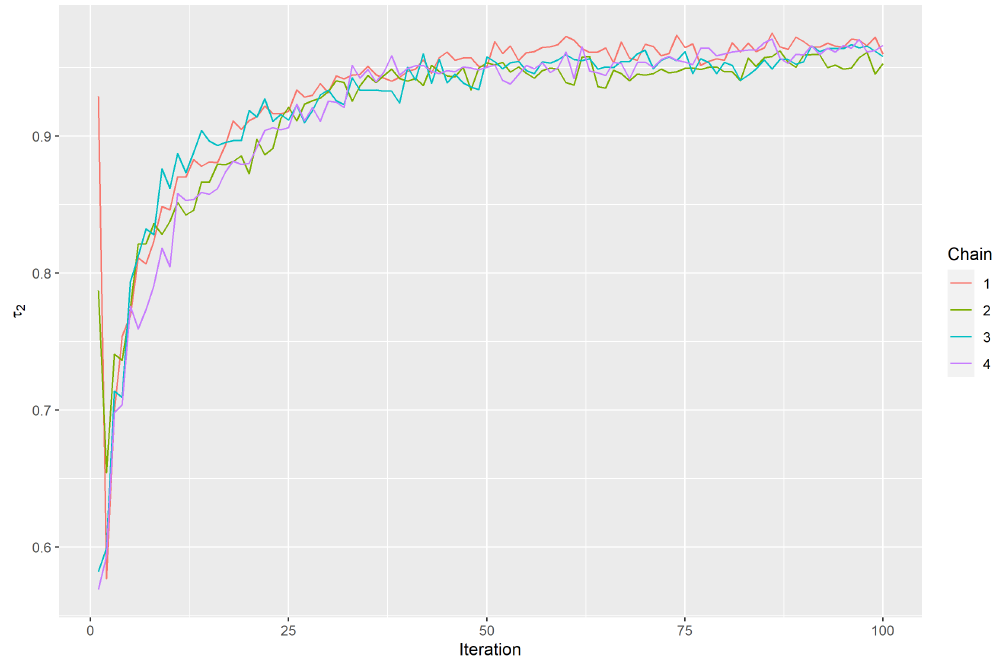
\includegraphics[width=\textwidth]{imgs/convergence.png}
\end{frame}

\begin{frame}
\frametitle{Markov Chain Monte Carlo}
\framesubtitle{Convergence}
\begin{itemize}
 \item{All chains should converge to the same distribution $\rightarrow$ traceplot}
\end{itemize}
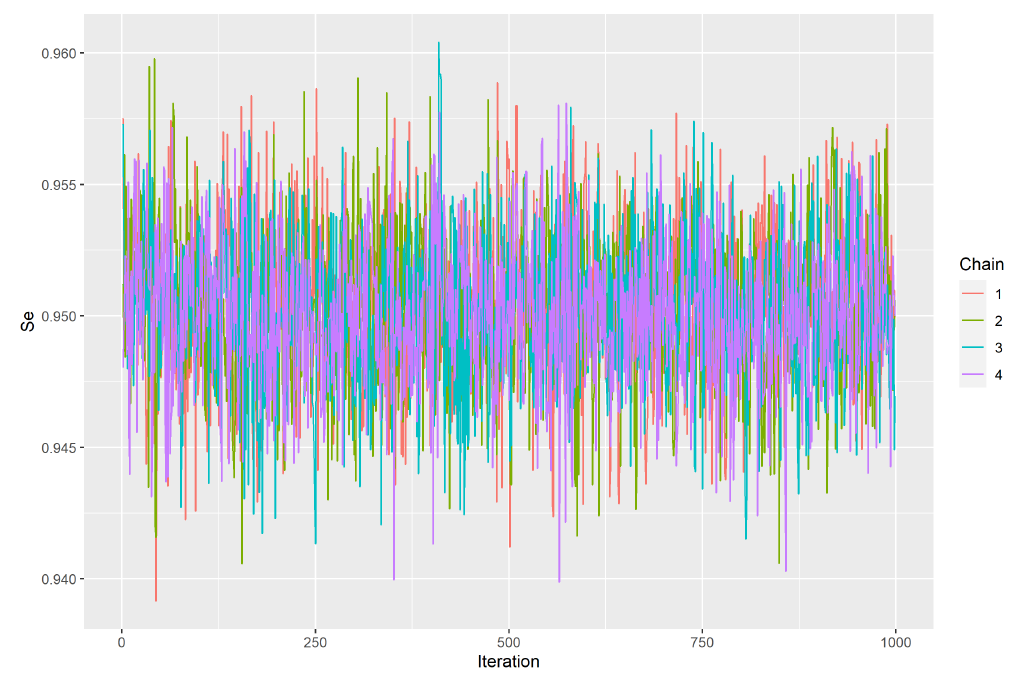
\includegraphics[width=\textwidth]{imgs/traceplot.png}
\end{frame}

\begin{frame}
\frametitle{Markov Chain Monte Carlo}
\framesubtitle{Convergence}
\begin{itemize}
 \item{Different chains can converge to different distributions}
 \begin{itemize}
  \item{Model with 5 parameters / each color is a chain}
 \end{itemize}
\end{itemize}
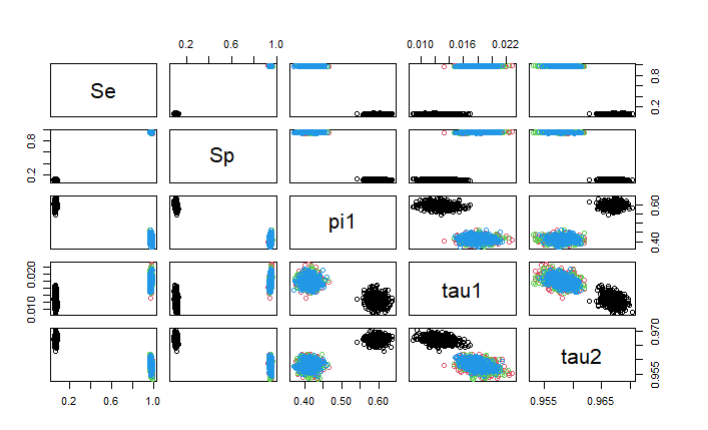
\includegraphics[width=\textwidth]{imgs/Stan_fail_1.png}
\end{frame}

\begin{frame}
\frametitle{Markov Chain Monte Carlo}
\framesubtitle{Autocorrelation}
\begin{itemize}
 \item{Autocorrelation: within a chain, high correlation between consecutive MCMC samples}
\end{itemize}
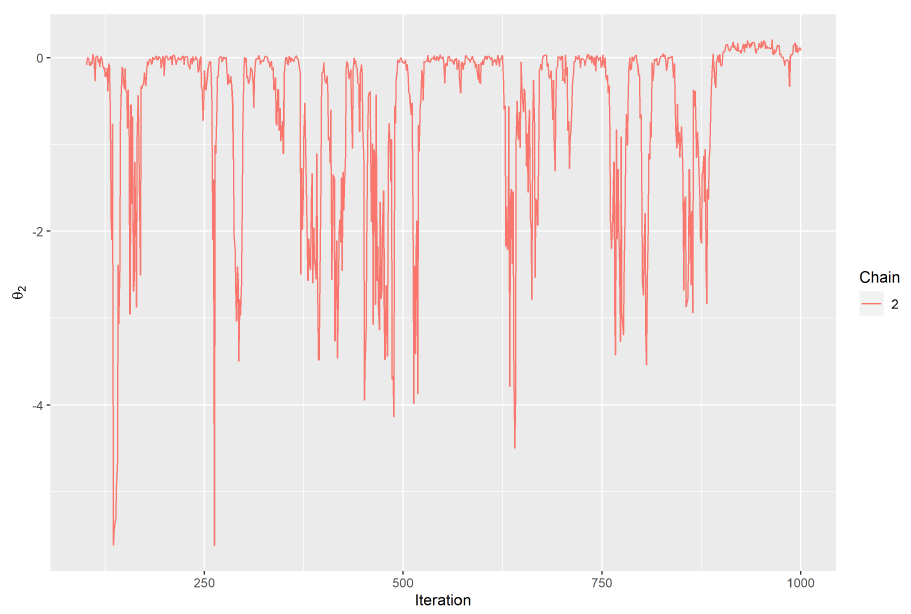
\includegraphics[width=\textwidth]{imgs/autocorrelation.png}

\end{frame}

\begin{frame}
\frametitle{Markov Chain Monte Carlo}
\framesubtitle{in pratcice}
\begin{itemize}
 \item{Run several chains ($> 2$): allows checking that the samples obtained do not come from different distributions = convergence (traceplots , Gelman Rubin statistic)}
 \item{Initialise each chain with different values}
 \item{Discard the first $n$ iterations = burn in, warmup}
 \item{If autocorrelation, use 1 out of $k$ iterations (depending on autocorrelation) = thinning}
\end{itemize}
\end{frame}

\begin{frame}
\frametitle{Markov Chain Monte Carlo}
\framesubtitle{Algorithms}
\begin{itemize}
  \item{There exist many different MCMC algorithms:}
 \begin{itemize}
  \item{Metropolis: first invented (1953)}
  \item[]{\scriptsize See an introduction here: \href{https:youtu.be/U561HGMWjcw}{Ben Lambert - An introduction to the Random Walk Metropolis algorithm}}
  \item{Metropolis Hastings}
  \item{Gibbs sampling: BUGS, WinBUGS, JAGS}
 \item{Hamiltonian Monte Carlo: Stan}
 \end{itemize}
\end{itemize}
\end{frame}

\begin{frame}
\frametitle{Markov Chain Monte Carlo}
\framesubtitle{Gibbs sampling}
\begin{itemize}
 \item{First widely used algorithm for Bayesian inference}
 \begin{itemize}
 \item{Not possible before the 1990s because computation intensive}
 \item{First implementations:}
  \begin{itemize}
   \item{BUGS = Bayesian Inference Using Gibbs Sampling}
   \item{WinBUGS , OpenBUGS}
  \end{itemize}
 \item{Most recent implementations}
  \begin{itemize}
   \item{\href{https://sourceforge.net/projects/mcmc-jags/files/}{JAGS}: Just Another Gibbs Sampler}
   \item{MultiBUGS}
   \item[$\Rightarrow$]{Same principles, more efficient}
  \end{itemize}
 \end{itemize}
\end{itemize}
\end{frame}

\begin{frame}
\frametitle{Markov Chain Monte Carlo}
\framesubtitle{Gibbs sampling}
\begin{itemize}
 \item{All the programmes use the same language to code statistical models}
 \item{Easy to write the code from model specification}
 \item{Straightforward to translate the STOC free model equations into code}
\end{itemize}
\end{frame}

\begin{frame}
\frametitle{Markov Chain Monte Carlo}
\framesubtitle{Hamiltonian Monte Carlo}
\begin{itemize}
 \item{Implemented in \href{https://mc-stan.org}{Stan}}
 \item{Much more efficient than Gibbs sampling}
 \begin{itemize}
  \item{Exploration of the posterior distribution much more efficient}
  \item{Less autocorrelation $\rightarrow$ requires less iterations}
 \end{itemize}
 \item{Does not support latent discrete parameters}
 \begin{itemize}
  \item{Not possible to code the STOC free model as simply as in JAGS}
 \end{itemize}
\end{itemize}
\end{frame}

\begin{frame}
\frametitle{Markov Chain Monte Carlo}
\framesubtitle{}

\begin{itemize}
 \item{For a visual comparison of different MCMC algorithms, see: \href{http://chi-feng.github.io/mcmc-demo/}{The Markov-chain Monte Carlo Interactive Gallery by Chi-Feng}}
\end{itemize}
\end{frame}

\section{Implementation}
\begin{frame}
\frametitle{Table of Contents}
  \tableofcontents[currentsection]
\end{frame} 

\subsection[JAGS]{The STOC free model in JAGS}

\begin{frame}
\frametitle{JAGS model}
\begin{itemize}
 \item{Easy to go from model equations to JAGS code}
 \item{On the following slides:}
 \begin{itemize}
  \item{Simplified version in which test results assumed available for all months}
  \item{The \emph{real} model allows for missing test results with a complicated system of loops. Same idea but harder to read}
  \item{When no test available, the dynamics drive status evolution}
 \end{itemize}
\end{itemize}
\end{frame}








\begin{frame}[fragile]
\frametitle{JAGS model}
\framesubtitle{First status}
\scriptsize
\begin{verbatim}
model{
  ## loop over all herds
  ## t1 is the vector of indices for first month of test in each herd
  ## t2 is the vector of indices for second month of test in each herd
  ## tf is the vector of indices for last month of test in each herd
  for(i in 1:N_herds){
    
    ### First monthly status of each herd
    ## probability of being latent status positive for herd i at t1
    logit_pi1[i] ~ dnorm(logit_pi1_mean, logit_pi1_prec)
    
    ## latent status for herd i at time = 1
    Status[t1[i]] ~ dbern(ilogit(logit_pi1[i]))
  
    ## probability of being test positive given herd status
    p_test_pos[t1[i]] <- Se * Status[t1[i]] + 
                         (1 - Sp) * (1 - Status[t1[i]])
    
    ## test result associated with first Status => data
    test_res[t1[i]] ~ dbern(p_test_pos[t1[i]])
...    
\end{verbatim}
\end{frame}


\begin{frame}[fragile]
\frametitle{JAGS model}
\framesubtitle{Statuses 2 to last - 1}
\scriptsize
\begin{verbatim}
    ### Statuses 2 to  1 minus last
    for(t in (t1[i] + 1):(tf[i] - 1)){
      
      # probability of new infection
      # logistic regression
      logit(tau1[t]) <- inprod(risk_factors[t,], theta)
      
      ## probability of being status positive given previous status,
      ## tau1 and tau2
      pi[t] <- (1 - Status[t - 1]) * tau1[t] +
                Status[t - 1] * tau2
      
      ## herd status at time t
      Status[t] ~ dbern(pi[t])
      
      ## probability of test positive at time t
      p_test_pos[t] <- Se * Status[t] + (1 - Sp) * (1 - Status[t])
      
      ## test result at time t  => data
      test_res[t] ~ dbern(p_test_pos[t])
      
    }
 \end{verbatim}
\end{frame}

\begin{frame}[fragile]
\frametitle{JAGS model}
\framesubtitle{Predicted statuses}
\scriptsize
\begin{verbatim}
    # probability of new infection
    logit(tau1[tf[i]]) <- inprod(risk_factors[tf[i],], theta)
    
    ## Predicted probability of infection for herd i on last month
    pi[tf[i]] <- tau1 * (1 - Status[tf[i] - 1]) + 
                 tau2 * Status[tf[i] - 1]
    # probability of infection updated with test result
    predicted_proba[tf[i]] <- test_res[tf[i]] * (  
      Se * pi[tf[i]] / (Se * pi[tf[i]] + (1 - Sp) * (1 - pi[tf[i]]))
    ) + (1 - test_res[tf[i]]) * (                  
        (1 - Se) * test_res[tf[i]] /
          ((1 - Se) * pi[tf[i]]  + Sp * (1 - pi[tf[i]] ) )
      )
    
  }
\end{verbatim}
\end{frame}

\begin{frame}[fragile]
\frametitle{JAGS model}
\framesubtitle{Priors}
\scriptsize
\begin{verbatim}
  ### Priors
  ## test characteristics
  Se ~ dbeta(Se_beta_a, Se_beta_b)
  Sp ~ dbeta(Sp_beta_a, Sp_beta_b)

  ## Status dynamics - sampling on the logit scale
  logit_tau2 ~ dnorm(logit_tau2_mean, logit_tau2_prec)

  ## logit back to the probability scale
  tau2 <- ilogit(logit_tau2)
  
  ## Logistic regression coefficients
  for(i_rf in 1:n_risk_factors){
    
    theta[i_rf] ~ dnorm(theta_norm_mean[i_rf], theta_norm_prec[i_rf])
    
  }
  
  }
\end{verbatim}
\end{frame}


\subsection[Stan]{The STOC free model in Stan}

\begin{frame}[fragile]
\frametitle{Stan model}
\begin{itemize}
 \item{Stan implements Hamiltonian Monte Carlo which is expected to be more efficient at sampling from the full posterior distribution}
 \item{Stan does not support latent discrete parameters}
 \item{Translation of the model’s equations not as easy as with JAGS}
 \item{Various HMM implementations in Stan described in a tutorial by \href{https://github.com/luisdamiano/stancon18}{Damiano et al. (2017)}}
\end{itemize}
\end{frame}

\begin{frame}
\frametitle{Stan model}
\begin{itemize}
 \item{Forward algorithm adapted from the tutorial}
 \item{Same model as the JAGS version, but estimation performed in a different way}
\end{itemize}
\end{frame}

\begin{frame}[fragile]
\frametitle{Stan model}
\framesubtitle{Declaration of variables}
\scriptsize
\begin{verbatim}
data{

  int<lower=1> n_herds;
  int<lower=1> herds_t1[n_herds];
  int<lower=1> herds_t2[n_herds];
  int<lower=1> herds_T[n_herds];
  int<lower=1> N;
  int<lower=0, upper=3> test_res[N];
  real<lower = 0> Se_beta_a;
  real<lower = 0> Se_beta_b;
  real<lower = 0> Sp_beta_a;
  real<lower = 0> Sp_beta_b;
  real logit_pi1_mean;
  real logit_pi1_sd;
  real logit_tau2_mean;
  real logit_tau2_sd;
  int<lower = 0> n_risk_factors;
  real theta_norm_mean[n_risk_factors];
  real theta_norm_sd[n_risk_factors];
  matrix[N, n_risk_factors] risk_factors;

}
\end{verbatim}
\end{frame}



\begin{frame}[fragile]
\frametitle{Stan model}
\framesubtitle{Parameters}
\scriptsize
\begin{verbatim}
parameters{

  real<lower = 0, upper = 1> Se;
  real<lower = 0, upper = 1> Sp;
  real<lower = 0, upper = 1> pi1;
  real<lower = 0, upper = 1> tau2;
  vector[n_risk_factors] theta;

}
\end{verbatim}
\end{frame}


\begin{frame}[fragile]
\frametitle{Stan model}
\framesubtitle{Transformed parameters}
\scriptsize
\begin{verbatim}
transformed parameters{

  // logalpha needs to be accessible to other blocks
  matrix[N, 2] logalpha;

  {

    // accumulator used at each time step
    real tau1[N];
    real accumulator[2];

    // logistic regression for tau1
  for(n in 1:N){

  tau1[n] = inv_logit(risk_factors[n,] * theta);

  }
\end{verbatim}

\end{frame}

\begin{frame}[fragile]
\frametitle{Stan model}
\framesubtitle{First status}
\scriptsize
\begin{verbatim}
    // looping over all herds
    for(h in 1:n_herds){

      // first test in sequence
      // negative status
      logalpha[herds_t1[h], 1] = log(1 - pi1) + 
                      bernoulli_lpmf(test_res[herds_t1[h]] | 1 - Sp);
      // positive status
      logalpha[herds_t1[h], 2] = log(pi1) + 
                      bernoulli_lpmf(test_res[herds_t1[h]] | Se);

 \end{verbatim}
\end{frame}


\begin{frame}[fragile]
\frametitle{Stan model}
\framesubtitle{Status transition / no test result}
\scriptsize
\begin{verbatim}
// tests 2 in T in sequence
  for(t in herds_t2[h]:herds_T[h]){

// Missing test result     
     if(test_res[t] == 3){

// transition from status negative to status negative (j = 1; i = 1)
     accumulator[1] = logalpha[t-1, 1] + log(1 - tau1[t]);
// transition from status positive to status negative (j = 1; i = 1)
     accumulator[2] = logalpha[t-1, 2] + log(1 - tau2);

     logalpha[t, 1] = log_sum_exp(accumulator);

// transition from status negative to status negative (j = 1; i = 1)
     accumulator[1] = logalpha[t-1, 1] + log(tau1[t]);
// transition from status positive to status positive (j = 1; i = 1)
     accumulator[2] = logalpha[t-1, 2] + log(tau2);

     logalpha[t, 2] = log_sum_exp(accumulator);

    } else {
 \end{verbatim}
\end{frame}


\begin{frame}[fragile]
\frametitle{Stan model}
\framesubtitle{Status transition / test result}
\scriptsize
\begin{verbatim}
// transition from status negative to status negative (j = 1; i = 1)
    accumulator[1] = logalpha[t-1, 1] + 
                     log(1 - tau1[t]) + 
                     bernoulli_lpmf(test_res[t] | 1 - Sp);
// transition from status positive to status negative (j = 1; i = 1)
    accumulator[2] = logalpha[t-1, 2] + 
                     log(1 - tau2) + 
                     bernoulli_lpmf(test_res[t] | 1 - Sp);

    logalpha[t, 1] = log_sum_exp(accumulator);
\end{verbatim}
\end{frame}


\begin{frame}[fragile]
\frametitle{Stan model}
\framesubtitle{Status transition / test result}
\scriptsize
\begin{verbatim}
// transition from status negative to status negative (j = 1; i = 1)
   accumulator[1] = logalpha[t-1, 1] + 
                    log(tau1[t]) + 
                    bernoulli_lpmf(test_res[t] | Se);
// transition from status positive to status positive (j = 1; i = 1)
   accumulator[2] = logalpha[t-1, 2] + 
                    log(tau2) + 
                    bernoulli_lpmf(test_res[t] | Se);

   logalpha[t, 2] = log_sum_exp(accumulator);

       } // if

     } // time sequence loop

    } // herd loop

  } //local

} // end of block
\end{verbatim}
\end{frame}


\begin{frame}[fragile]
\frametitle{Stan model}
\framesubtitle{Priors and likelihood}
\scriptsize
\begin{verbatim}
model{

// priors for test characteristics
     Se ~ beta(Se_beta_a, Se_beta_b);
     Sp ~ beta(Sp_beta_a, Sp_beta_b);

// priors for status dynamics
  logit(pi1) ~ normal(logit_pi1_mean, logit_pi1_sd);
  logit(tau2) ~ normal(logit_tau2_mean, logit_tau2_sd);

// priors for the logistic regression coefficients
  for(k in 1:n_risk_factors){

  theta[k] ~ normal(theta_norm_mean[k], theta_norm_sd[k]);

  }

// update based only on last logalpha of each herd
  for(i in 1:n_herds)
    target += log_sum_exp(logalpha[herds_T[i]]);

}
\end{verbatim}
\end{frame}


\begin{frame}[fragile]
\frametitle{Stan model}
\framesubtitle{Predicted status}
\scriptsize
\begin{verbatim}
generated quantities{

  // variable in which predictions are stored
  real pred[n_herds];

  {
    matrix[n_herds, 2] alpha;

  // loop in which the probabilities of infection are predicted
    for(i in 1:n_herds){
      alpha[i] = softmax(logalpha[herds_T[i],]')';
      pred[i] = alpha[i, 2];
    }
  }
}
\end{verbatim}
\end{frame}


\subsection[JAGS vs. Stan]{Comparison of the JAGS and Stan implementations}

\begin{frame}
\frametitle{Comparison of the JAGS and Stan implementations}
\begin{itemize}
 \item{The JAGS and Stan implementations of the model were compared using data collected as part of BVDV control programme in France}
 \begin{itemize}
  \item{Work under review with \href{https://animsci.peercommunityin.org/}{PCI Animal Science}, available as a \href{https://www.biorxiv.org/content/10.1101/2020.07.10.197426v4.full}{pre-print}.}
 \end{itemize}
 \item{The Stan implementation:}
 \begin{itemize}
  \item{gives the same parameter estimates}
  \item{is much faster}
  \item{converges much better}
  \item{returns predicted probabilities of infection that are easier to interpret}
 \end{itemize}
\end{itemize}
\end{frame}

\subsection{\texttt{STOCfree} package}

\begin{frame}
\frametitle{The \texttt{STOCfree} R package}
\framesubtitle{What is an R package?}
\begin{itemize}
\item[]{
\includegraphics[width=.07\textwidth]{imgs/Rlogo.png}}
\begin{itemize}
 \item{Programming environment for data manipulation and analysis}
 \item{Widely used}
 \item{Free}
\end{itemize}
\item[]{
\includegraphics[width=.07\textwidth]{imgs/Rlogo.png} package}
 \begin{itemize}
  \item{Set of functions gathered to perform specific tasks}
  \item{Users install a package and can use the functions they contain}
  \item{Packages are installed from the web (CRAN, GitHub…)}
 \end{itemize}
\end{itemize}
\end{frame}

\begin{frame}
\frametitle{The \texttt{STOCfree} R package}
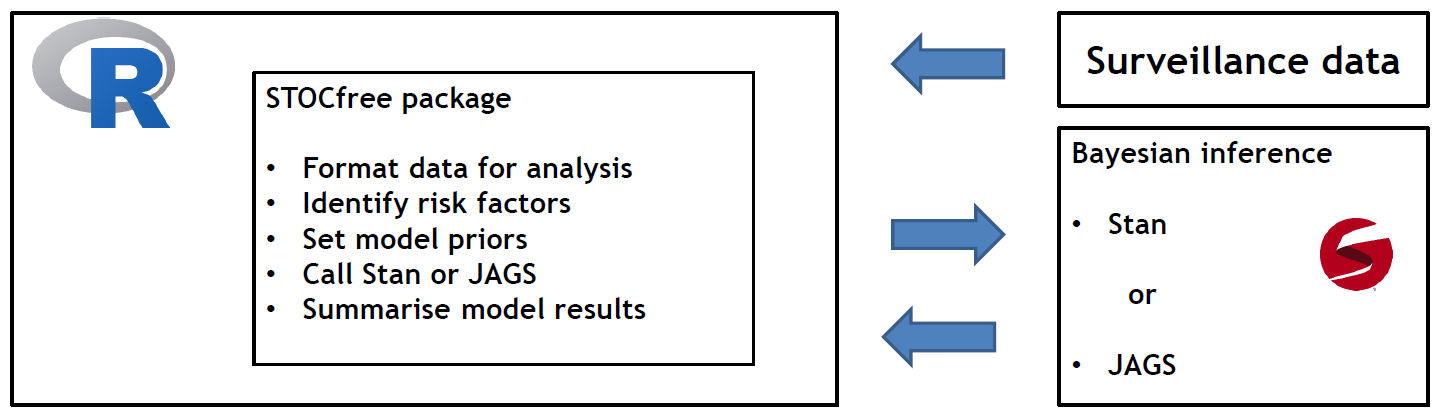
\includegraphics[width=\textwidth]{imgs/STOCfree_package.png}
\end{frame}

\begin{frame}
\frametitle{The \texttt{STOCfree} R package on Github}
\begin{itemize}
 \item{The package is hosted on Github}
 \url{https://github.com/AurMad/STOCfree}
 \item{Github is a server hosting:}
 \begin{itemize}
  \item{The package code}
  \item{The package documentation}
  \item{The history of development and different package versions, using the Git versioning programme}
 \end{itemize}
\end{itemize}
\end{frame}

\begin{frame}
\frametitle{The STOCfree R package on Github}
\begin{itemize}
 \item{All the code is in the \texttt{R} folder}
\end{itemize}
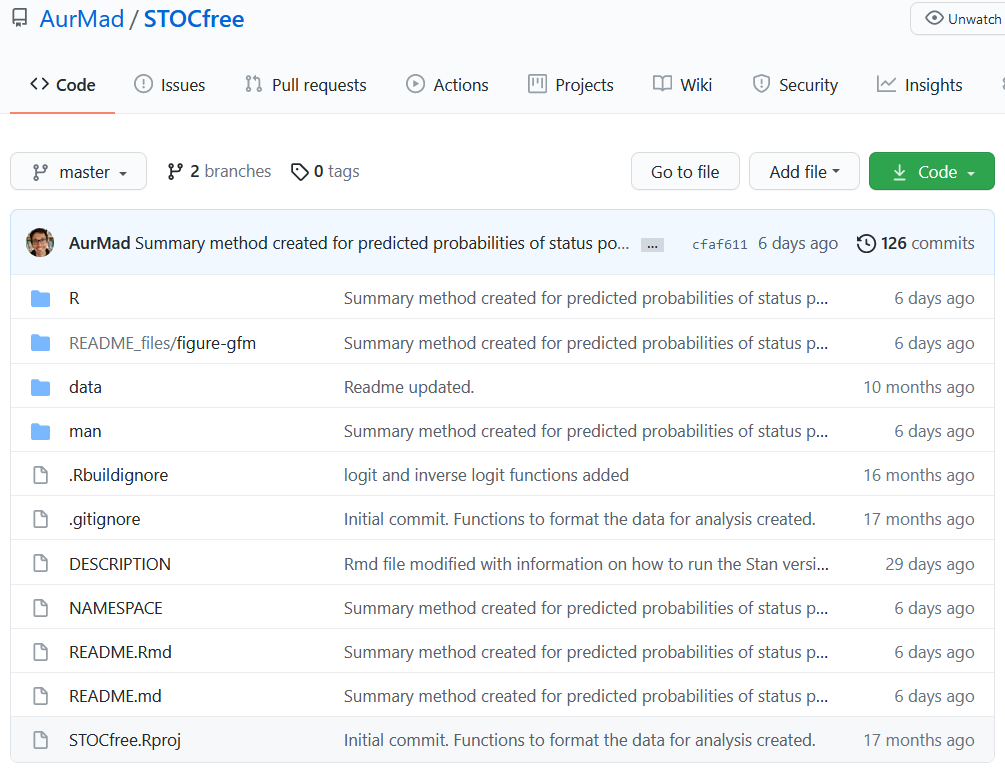
\includegraphics[width=.9\textwidth]{imgs/STOCfree_Github.png}
\end{frame}

\begin{frame}
\frametitle{The STOCfree R package on Github}
\begin{itemize}
 \item{The documentation is at the bottom of the page}
\end{itemize}
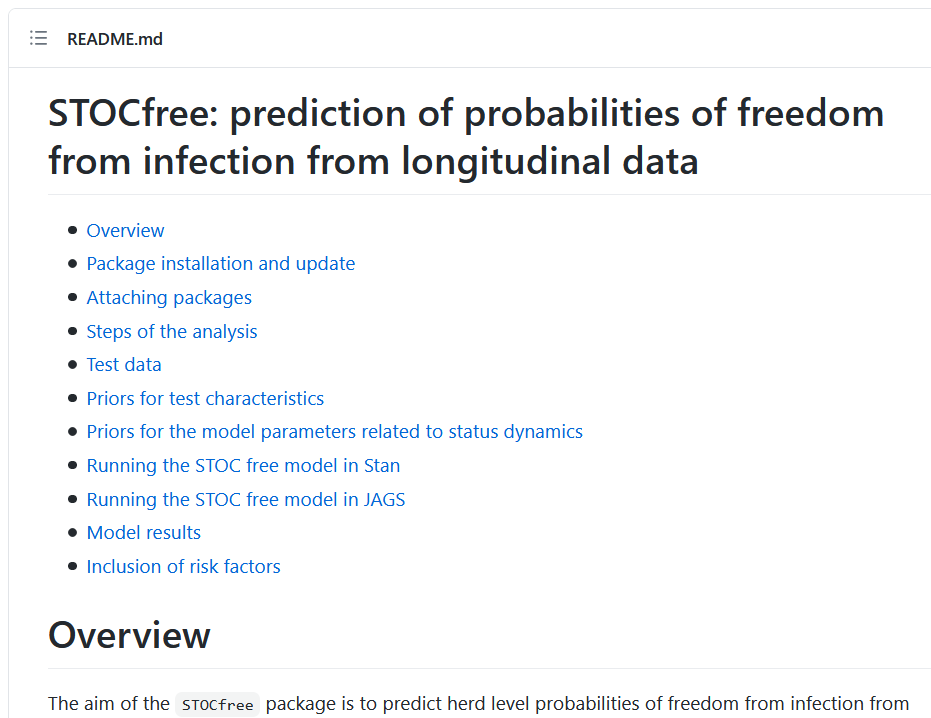
\includegraphics[width=.9\textwidth]{imgs/STOCfree_Github_1.png}
\end{frame}

{
    \usebackgroundtemplate{
\includegraphics[height=\paperheight,width=\paperwidth]{imgs/last_slide.png}}
    \setbeamertemplate{navigation symbols}{}
    \begin{frame}[plain]
    \end{frame}
    }

\end{document}
